\chapter{Data Structures}
\label{chap:struct}
\biglet{I}{n} this section, I describe the structure of the \emph{reducer tree} as well as all types of \emph{reducer nodes} implemented in our framework. We also show the structure of individual \emph{tuners} and how they can be arranged into the \emph{tuner network}.

\section{The Reducer Tree}
 Estimating material assignments at output device resolution is computationally intractable. Therefore, material assignment has to be computed using a reduced representation. We specify this representation using a \emph{reducer tree}. This structure is conceptually similar to those used in programmable shading systems (such as Cook's shade trees~\shortcite{Cook1984} or Maya Shader Networks). These systems are primarily concerned with assigning known materials and textures to an object's surface whereas we are seeking an optimal volumetric assignment from a defined set of materials. In order to accomplish this task, we build a tree-based data structure which contains the entire object volume as its root node. We define two classes of \emph{reducer nodes}: \emph{geometry nodes} and \emph{material nodes}.

\paragraph{Geometry Nodes:}A \emph{geometry node} takes a volumetric region as input and produces a partition of this region into smaller sub-regions. 
These can be attached to the object geometry or they can be defined in a global coordinate system.
To demonstrate the flexibility of the \emph{reducer tree}, we define a small yet powerful set of partitioning nodes which are described as follows %used in our prototype
 (\autoref{fig:geometryNodes}):\vspace{-0.25\baselineskip}
\begin{itemize}
\item Plane Node --  partitions the space into two half-spaces, \vspace{-0.25\baselineskip}
\item Column Node -- takes as input the number of columns and accordingly partitions the space,\vspace{-0.25\baselineskip}
\item Voxel Node -- takes as input voxel size and uniformly partitions the space,\vspace{-0.25\baselineskip}
\item B-spline Node -- partitions a volume into two regions cut by a B-spline,\vspace{-0.25\baselineskip}
\item Stratum Node -- takes a single positive distance parameter as an input and partitions the volume into two regions divided by the iso-distance surface.\vspace{-0.25\baselineskip}
\end{itemize} 

\begin{figure}[h]
\centering
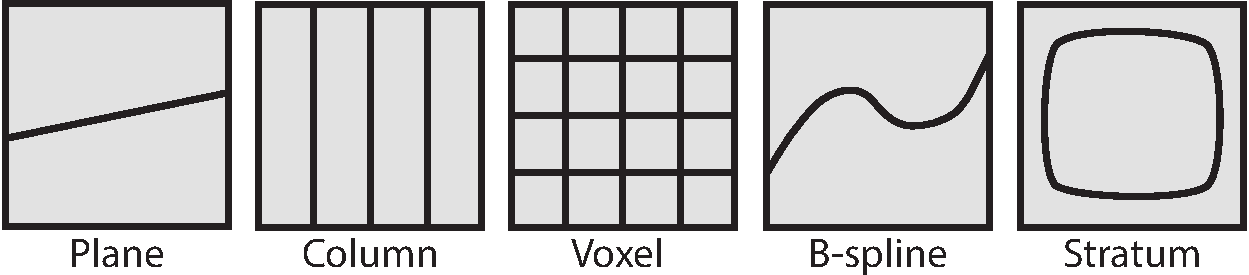
\includegraphics[width=0.7\linewidth]{figure/geometryNodes}
\caption{2D representations  of the \emph{geometry nodes} used in our \emph{reducer tree}.}
\label{fig:geometryNodes}
\end{figure}

\paragraph{Material Nodes:} The \emph{leaf nodes} of the \emph{reducer tree} are the material parameterization nodes. These contain a material assignment function $\lambda\left(x\right)$ that maps spatial coordinates to materials. We allow our \emph{material nodes} to assign a void material to regions of the volume. Hence, surface displacements and material assignments can be treated in a unified fashion.
While \emph{material node} can be extended to implement arbitrary material assignment functions (such as Functionally Graded Materials), all the following results require only a single type of \emph{material node}, \emph{layered node}, which assigns $k$ material layers of varying thickness to a geometry partition. We can even assign a constant material to a region using a \emph{layered node} with a single layer. 

\emph{Geometry nodes} and \emph{material nodes} can be connected into a tree structure that describes a material assignment function throughout the input geometry. 
The essential property of this data structure is that it naturally adapts to the input geometry. This key feature allows it to be reused for different shapes.
\autoref{fig:red1} shows two examples of \emph{reducer trees} and the resulting geometric distributions of materials.
Since the tree describes a nested set of partitions, we can efficiently perform material queries by passing a query point through the tree until it arrives at a parameterization node. 
We note that the \emph{reducer tree} does not inherently enforce material continuity between disjoint regions of the object; however, for material assignment problems, this is neither required nor desired. 

\begin{figure}[h]
\centering
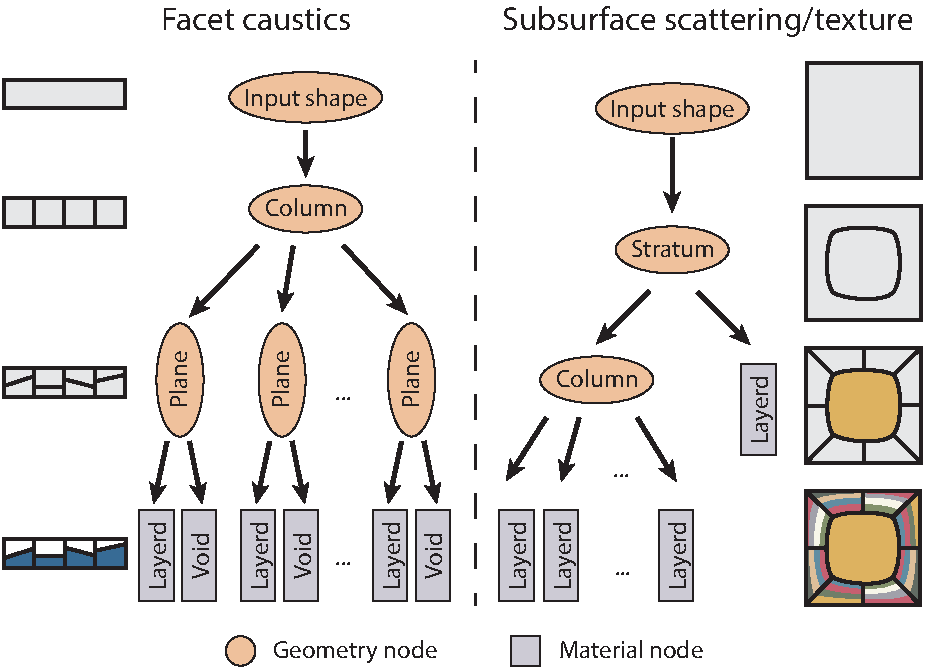
\includegraphics[width=0.7\linewidth]{figure/redNetworkNew.pdf}
\caption{Two examples of our \emph{reducer tree}. Left: in order to create an object producing a caustic, the input shape is first divided into columns. Next, each column is sliced by a plane.
By assigning materials to lower parts of the columns, the microfacet surface is created.
Right: a textured object with subsurface scattering properties is produced by first dividing the input shape using a \emph{stratum node}. Then, the outer layer is sliced into columns, which create a texture once materials are assigned. The inner part of the object obtains a material with given subsurface scattering properties.  
}
\label{fig:red1}
\end{figure}

\section{Tuners and Tuning the Reducer Tree}
We define \emph{tuners} as an abstract interface between a \emph{reducer node} and an optimization algorithm. 
A \emph{reducer node} has parameters that control its space partitioning and material composition, e.g., \emph{stratum node} has a parameter which determines its thickness, \emph{column node} has parameters that control the width of columns.
A \emph{tuner} is responsible for tuning these parameters to achieve a specified goal.
A \emph{tuner} is comprised of an optimization scheme, an error metric, a simulator and a goal (\autoref{fig:tuner0}). 
In order to create an optimal material assignment, \emph{tuner nodes} must be attached to the \emph{reducer tree}. The developer links each \emph{tuner} to a \emph{reducer node} in the \emph{reducer tree}. Each \emph{tuner} then traverses the \emph{reducer subtree} (rooted at this \emph{reducer node}) and constructs a parameter list by querying each visited \emph{reducer node}. The developer can label parameters as fixed or free. \emph{Tuner nodes} contain specific optimization routines (e.g., a quadratic program solver). The \emph{tuner node} then uses this routine to optimize its associated free parameters. During execution, additional information (e.g., parameters, errors, etc.) from neighboring Tuner Nodes can be obtained via the \emph{tuner network} (Section~\ref{sec:TunerNetwork}).  Tuner execution can be scheduled (again by the programmer) allowing both serial and parallel processing. 

\autoref{fig:combine} (left) shows a simple example in which two \emph{tuners} are attached to sibling nodes in a \emph{reducer tree}. The first \emph{tuner} is responsible for \emph{layered} and \emph{void material nodes }while the second is responsible for several \emph{layered material nodes}.  

\begin{figure}[h]
\centering
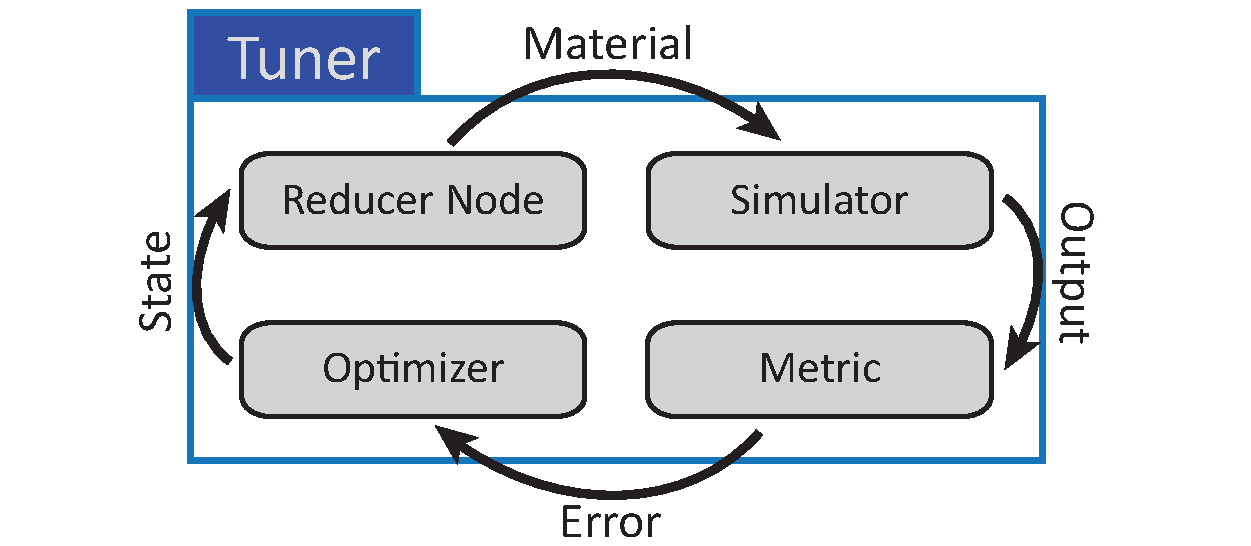
\includegraphics[width=0.7\linewidth]{figure/tuner2.pdf}
\caption{A diagram of the \emph{tuner} workflow. Arrows indicate flow and type of information passed between the individual \emph{tuner} components.}
\label{fig:tuner0}
\end{figure}

\section{Tuner Network}
\label{sec:TunerNetwork}
For many fabrication problems, \emph{tuners} should not act in isolation. For instance, an optimal material assignment at a given point depends on the material assignment in the neighborhood. Tuning the free parameters without taking into account this dependency usually yields suboptimal results. Therefore, we allow the \emph{tuners} to share information according to a user-specified graph structure. This allows our framework to interface with a wide range of existing graph-based optimization and inference algorithms. For example, Figure~\ref{fig:combine} (right) shows one of the \emph{tuner networks} used in our experiments.
In this network, each node is connected to its four neighbors. In Figure~\ref{fig:ReducerTreesAdditional}, \emph{tuners} enclosed in dashed boxes are connected in this form. \emph{Tuner networks} do not always exhibit this regular connectivity. For instance, \emph{tuners} can be completely unconnected (\autoref{fig:combine} (left) or be organized into groups which feature intra- but not inter-group connections.

\begin{figure}[h]
\centering
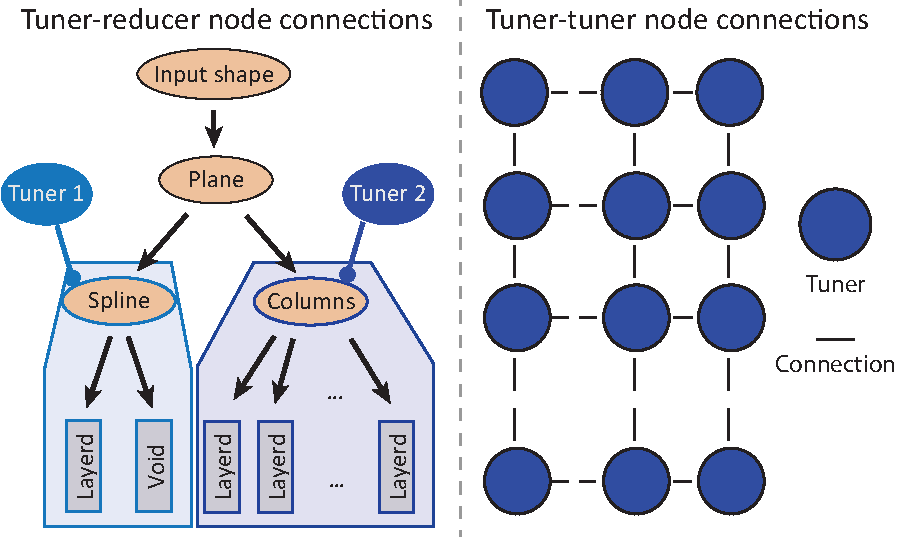
\includegraphics[width=0.7\linewidth]{figure/tunedrt.pdf}
\caption{ 
	Left: Two \emph{tuners} attached to a \emph{reducer tree}. Each \emph{tuner} is responsible for tuning the nodes in its attached subtree (denoted by shapes with similarly colored outlines). 
	Right: One type of \emph{tuner network} used in our experiments.}
\label{fig:combine}
\end{figure}
